\documentclass[answers,12pt,addpoints]{exam} 
\usepackage{import}

\import{C:/Users/prana/OneDrive/Desktop/MathNotes}{style.tex}

% Header
\newcommand{\name}{Pranav Tikkawar}
\newcommand{\course}{Stochastic Processes}
\newcommand{\assignment}{Homework 4}
\author{\name}
\title{\course \ - \assignment}

\begin{document}
\maketitle

\section*{Problem 1: Detailed balance of the random-scan Gibbs sampler}

Let
\[
\Omega = \Omega_1 \times \cdots \times \Omega_d
\]
be a finite product space, where each $\Omega_i$ is a finite set. Let $\pi$ be a probability distribution on $\Omega$ such that $\pi(x) > 0$ for every $x \in \Omega$.

For a state $x = (x_1, \ldots, x_d) \in \Omega$, write
\[
x_{-i} = (x_1, \ldots, x_{i-1}, x_{i+1}, \ldots, x_d)
\]
for the collection of all coordinates except the $i$-th one.

We consider the following random-scan Gibbs sampler: given the current state $X_t = x$,
\begin{enumerate}
\item choose an index $I_t \in \{1, \ldots, d\}$ uniformly at random;
\item update only the $I_t$-th coordinate by drawing
\[
X^{(I_t)}_{t+1} \sim \pi(\,\cdot \mid X^{(-I_t)}_t\,),
\]
while keeping all other coordinates unchanged.
\end{enumerate}
In other words, if $I_t = i$, then $X_{t+1}$ is obtained from $X_t$ by resampling the $i$-th coordinate from the conditional distribution
\[
\pi(\,\cdot \mid x_{-i}\,).
\]

\begin{enumerate}
\item Show that if $x$ and $y$ differ in more than one coordinate, then $P(x,y) = 0$.
\begin{solution}
Recall that in one step of the random-scan Gibbs sampler, we first choose an index
$I_t \in \{1,\dots,d\}$ uniformly at random, and then update only the $I_t$-th
coordinate using the conditional distribution $\pi(\,\cdot \mid x_{-I_t})$,
leaving all other coordinates unchanged.

Let $x,y \in \Omega$ be two states that differ in more than one coordinate.
Then for every index $i \in \{1,\dots,d\}$, one of the following holds:
\begin{itemize}
\item either $x_j \neq y_j$ for some $j \neq i$, in which case it is impossible
to obtain $y$ from $x$ by changing only coordinate $i$ and keeping all other
coordinates fixed;
\item or $x_i \neq y_i$ and there exists $j \neq i$ with $x_j \neq y_j$, so again
$y$ cannot be obtained by changing a single coordinate of $x$.
\end{itemize}
Thus, conditional on any choice $I_t = i$, the probability that $X_{t+1} = y$
given $X_t = x$ is zero, because the transition from $x$ to $y$ would require
changing more than one coordinate in a single step.

Since the index $I_t$ is the only random choice that determines which coordinate
is updated, and for each $i$ the probability of transitioning from $x$ to $y$ in
one step is zero, we have
\[
P(x,y) = \mathbb{P}(X_{t+1} = y \mid X_t = x)
= \sum_{i=1}^d \mathbb{P}(I_t = i)\,
\mathbb{P}(X_{t+1} = y \mid X_t = x, I_t = i)
= 0.
\]
Hence, if $x$ and $y$ differ in more than one coordinate, then $P(x,y) = 0$, as
required.
\end{solution}
\item Suppose $x$ and $y$ differ in exactly one coordinate, say the $i$-th one, and satisfy
\[
x_{-i} = y_{-i}.
\]
Show that
\[
P(x,y) = \frac{1}{d}\,\pi(y_i \mid x_{-i}).
\]

\begin{solution}
Suppose $x,y \in \Omega$ differ in exactly one coordinate, say the $i$-th one, and
satisfy $x_{-i} = y_{-i}$. Then the only way to move from $x$ to $y$ in one step
of the random-scan Gibbs sampler is:
\begin{itemize}
\item first choose $I_t = i$ in step 1, which happens with probability
$\mathbb{P}(I_t = i) = 1/d$;
\item then, in step 2, resample the $i$-th coordinate from the conditional
distribution $\pi(\,\cdot \mid x_{-i})$ and obtain the value $y_i$.
\end{itemize}
If $I_t \neq i$, the $i$-th coordinate of $X_t$ is not updated, so we cannot have
$X_{t+1} = y$ because $x_i \neq y_i$. Thus,
\[
P(x,y)
= \mathbb{P}(X_{t+1} = y \mid X_t = x)
= \mathbb{P}(I_t = i)\,
\mathbb{P}(X_{t+1} = y \mid X_t = x, I_t = i).
\]
Given $X_t = x$ and $I_t = i$, we update only the $i$-th coordinate using
$\pi(\,\cdot \mid x_{-i})$ and keep all other coordinates fixed at $x_{-i} =
y_{-i}$. Therefore,
\[
\mathbb{P}(X_{t+1} = y \mid X_t = x, I_t = i)
= \mathbb{P}(X_{t+1,i} = y_i \mid X_t = x, I_t = i)
= \pi(y_i \mid x_{-i}).
\]
Combining these two factors, we obtain
\[
P(x,y) = \frac{1}{d}\,\pi(y_i \mid x_{-i}),
\]
as claimed.
\end{solution}
\item Prove that the Gibbs sampler satisfies the detailed balance condition with respect to $\pi$, namely
\[
\pi(x) P(x,y) = \pi(y) P(y,x)
\quad \text{for all } x,y \in \Omega.
\]
\begin{solution}
We need to show that for all $x,y \in \Omega$,
\[
\pi(x) P(x,y) = \pi(y) P(y,x).
\]
We consider three cases.

\medskip
\noindent\textbf{Case 1: $x$ and $y$ differ in more than one coordinate.}
By part (1), $P(x,y) = 0$, and by the same argument with $x$ and $y$ swapped,
$P(y,x) = 0$. Hence
\[
\pi(x) P(x,y) = \pi(x)\cdot 0 = 0
\quad\text{and}\quad
\pi(y) P(y,x) = \pi(y)\cdot 0 = 0,
\]
so the detailed balance identity holds.

\medskip
\noindent\textbf{Case 2: $x = y$.}
In this case,
\[
\pi(x) P(x,x) = \pi(x) P(x,x),
\]
so the identity is trivially true.

\medskip
\noindent\textbf{Case 3: $x$ and $y$ differ in exactly one coordinate.}
Suppose $x$ and $y$ differ only in the $i$-th coordinate, and that
$x_{-i} = y_{-i}$. By part (2),
\[
P(x,y) = \frac{1}{d} \,\pi(y_i \mid x_{-i}),
\qquad
P(y,x) = \frac{1}{d} \,\pi(x_i \mid y_{-i}).
\]
Since $x_{-i} = y_{-i}$, we use the definition of conditional probability to write
\[
\pi(y_i \mid x_{-i})
= \frac{\pi(y_i,\, x_{-i})}{\pi(x_{-i})}
= \frac{\pi(y)}{\pi(x_{-i})},
\qquad
\pi(x_i \mid y_{-i})
= \frac{\pi(x_i,\, y_{-i})}{\pi(y_{-i})}
= \frac{\pi(x)}{\pi(y_{-i})}.
\]
Substituting $y_{-i} = x_{-i}$ in the second expression,
\[
\pi(y_i \mid x_{-i}) = \frac{\pi(y)}{\pi(x_{-i})},
\qquad
\pi(x_i \mid y_{-i}) = \frac{\pi(x)}{\pi(x_{-i})}.
\]
Therefore,
\[
\pi(x)\,P(x,y)
= \pi(x)\cdot\frac{1}{d}\cdot\frac{\pi(y)}{\pi(x_{-i})}
= \frac{\pi(x)\,\pi(y)}{d\,\pi(x_{-i})},
\]
and
\[
\pi(y)\,P(y,x)
= \pi(y)\cdot\frac{1}{d}\cdot\frac{\pi(x)}{\pi(x_{-i})}
= \frac{\pi(x)\,\pi(y)}{d\,\pi(x_{-i})}.
\]
These two expressions are equal, hence
\[
\pi(x) P(x,y) = \pi(y) P(y,x)
\]
whenever $x$ and $y$ differ in exactly one coordinate.

\medskip
Combining the three cases, we conclude that the random-scan Gibbs sampler
satisfies the detailed balance condition with respect to $\pi$.
\end{solution}
\item Conclude that $\pi$ is a stationary distribution of the random-scan Gibbs sampler.
\begin{solution}
From part (3), we know that $\pi$ satisfies the detailed balance condition
with respect to the transition kernel $P$:
\[
\pi(x) P(x,y) = \pi(y) P(y,x)
\quad \text{for all } x,y \in \Omega.
\]
To show that $\pi$ is stationary, we must prove that for every $y \in \Omega$,
\[
\sum_{x \in \Omega} \pi(x) P(x,y) = \pi(y).
\]
Using detailed balance, we have
\[
\sum_{x \in \Omega} \pi(x) P(x,y)
= \sum_{x \in \Omega} \pi(y) P(y,x)
= \pi(y) \sum_{x \in \Omega} P(y,x).
\]
Since $P$ is a Markov transition kernel, each row of $P$ sums to one, so
\[
\sum_{x \in \Omega} P(y,x) = 1.
\]
Therefore,
\[
\sum_{x \in \Omega} \pi(x) P(x,y)
= \pi(y) \cdot 1
= \pi(y),
\]
which shows that $\pi$ is a stationary distribution of the random-scan Gibbs
sampler.
\end{solution}
\end{enumerate}

%%%%%%%%%%%%%%%%%%%%%%%%%%%%%%%%%%%%%%%%%%%%%%%%
\section*{Problem 2: A $2\times 2$ Ising model}

Let the state space be
\[
\Omega = \{(1,1), (1,-1), (-1,1), (-1,-1)\},
\]
and define the target distribution
\[
\pi_\beta(\sigma) \propto \exp\bigl( \beta\, \sigma_1 \sigma_2 \bigr), \qquad \beta \ge 0,
\]
where $\sigma \in \{-1,1\}^2$.

This is the Ising model on a graph with one edge and no external field. Write
\[
\rho \;\stackrel{\text{def}}{=}\; \tanh \beta.
\]

\begin{enumerate}
\item Calculate $P(\sigma_1 \mid \sigma_2 = 1)$ and $P(\sigma_1 \mid \sigma_2 = -1)$.
\begin{solution}
The target distribution on $\sigma = (\sigma_1,\sigma_2) \in \{-1,1\}^2$ is
\[
\pi_\beta(\sigma) \propto \exp\bigl(\beta \sigma_1 \sigma_2\bigr).
\]
To compute the conditional distribution of $\sigma_1$ given $\sigma_2$, we
treat $\sigma_2$ as fixed and compare the two possible values
$\sigma_1 \in \{-1,1\}$.

\medskip
\noindent\textbf{Case $\sigma_2 = 1$.}
Then for $\sigma_1 = 1$,
\[
\pi_\beta(\sigma_1=1 \mid \sigma_2=1)
\;\propto\;
\exp\bigl(\beta \cdot 1 \cdot 1\bigr)
= e^{\beta},
\]
and for $\sigma_1 = -1$,
\[
\pi_\beta(\sigma_1=-1 \mid \sigma_2=1)
\;\propto\;
\exp\bigl(\beta \cdot (-1) \cdot 1\bigr)
= e^{-\beta}.
\]
Normalizing,
\[
\mathbb{P}(\sigma_1 = 1 \mid \sigma_2 = 1)
= \frac{e^{\beta}}{e^{\beta} + e^{-\beta}}
= \frac{e^{2\beta}}{e^{2\beta} + 1},
\qquad
\mathbb{P}(\sigma_1 = -1 \mid \sigma_2 = 1)
= \frac{e^{-\beta}}{e^{\beta} + e^{-\beta}}
= \frac{1}{e^{2\beta} + 1}.
\]

\medskip
\noindent\textbf{Case $\sigma_2 = -1$.}
Then for $\sigma_1 = 1$,
\[
\pi_\beta(\sigma_1=1 \mid \sigma_2=-1)
\;\propto\;
\exp\bigl(\beta \cdot 1 \cdot (-1)\bigr)
= e^{-\beta},
\]
and for $\sigma_1 = -1$,
\[
\pi_\beta(\sigma_1=-1 \mid \sigma_2=-1)
\;\propto\;
\exp\bigl(\beta \cdot (-1) \cdot (-1)\bigr)
= e^{\beta}.
\]
Normalizing,
\[
\mathbb{P}(\sigma_1 = 1 \mid \sigma_2 = -1)
= \frac{e^{-\beta}}{e^{\beta} + e^{-\beta}}
= \frac{1}{e^{2\beta} + 1},
\qquad
\mathbb{P}(\sigma_1 = -1 \mid \sigma_2 = -1)
= \frac{e^{\beta}}{e^{\beta} + e^{-\beta}}
= \frac{e^{2\beta}}{e^{2\beta} + 1}.
\]
Equivalently, in terms of $\rho = \tanh \beta$, these can be written as
\[
\mathbb{P}(\sigma_1 = s \mid \sigma_2 = t)
= \frac{1}{2}\bigl(1 + s t\, \rho\bigr),
\qquad s,t \in \{-1,1\}.
\]
\end{solution}
\item Write down the $4 \times 4$ transition matrix for the (random-scan) Gibbs sampler for this model.
\begin{solution}
We use the random-scan Gibbs sampler which, at each step, chooses one of the
two coordinates uniformly at random and updates it from its conditional
distribution given the other coordinate.

Let us fix the state ordering
\[
s_1 = (1,1),\quad s_2 = (1,-1),\quad s_3 = (-1,1),\quad s_4 = (-1,-1).
\]
We also write the conditional probabilities from part (a) as
\[
\mathbb{P}(\sigma_1 = s \mid \sigma_2 = t)
= \frac{1}{2}\bigl(1 + s t\, \rho\bigr),\qquad
\mathbb{P}(\sigma_2 = t \mid \sigma_1 = s)
= \frac{1}{2}\bigl(1 + s t\, \rho\bigr),
\]
for $s,t \in \{-1,1\}$, where $\rho = \tanh \beta$.

For each current state $x$, the next state $y$ is obtained by:
\begin{itemize}
\item with probability $1/2$, updating $\sigma_1$ given $\sigma_2$;
\item with probability $1/2$, updating $\sigma_2$ given $\sigma_1$.
\end{itemize}
We now compute each row of the $4\times 4$ transition matrix $P$.

\medskip
\noindent\textbf{From $s_1=(1,1)$.}
\begin{itemize}
\item Update $\sigma_1$ (prob.\ $1/2$): given $\sigma_2=1$,
\[
\mathbb{P}(\sigma_1=1\mid\sigma_2=1)=\frac{1+\rho}{2},\quad
\mathbb{P}(\sigma_1=-1\mid\sigma_2=1)=\frac{1-\rho}{2}.
\]
Thus,
\[
\mathbb{P}((1,1)\to(1,1) \text{ via }\sigma_1) = \frac{1+\rho}{2},\quad
\mathbb{P}((1,1)\to(-1,1) \text{ via }\sigma_1) = \frac{1-\rho}{2}.
\]
\item Update $\sigma_2$ (prob.\ $1/2$): given $\sigma_1=1$,
\[
\mathbb{P}(\sigma_2=1\mid\sigma_1=1)=\frac{1+\rho}{2},\quad
\mathbb{P}(\sigma_2=-1\mid\sigma_1=1)=\frac{1-\rho}{2}.
\]
Thus,
\[
\mathbb{P}((1,1)\to(1,1) \text{ via }\sigma_2) = \frac{1+\rho}{2},\quad
\mathbb{P}((1,1)\to(1,-1) \text{ via }\sigma_2) = \frac{1-\rho}{2}.
\]
\end{itemize}
Combining the two possibilities (each with weight $1/2$),
\[
P_{11} = \frac{1}{2}\cdot\frac{1+\rho}{2} + \frac{1}{2}\cdot\frac{1+\rho}{2}
= \frac{1+\rho}{2},
\]
\[
P_{12} = \frac{1}{2}\cdot 0 + \frac{1}{2}\cdot\frac{1-\rho}{2}
= \frac{1-\rho}{4},
\quad
P_{13} = \frac{1}{2}\cdot\frac{1-\rho}{2} + \frac{1}{2}\cdot 0
= \frac{1-\rho}{4},
\quad
P_{14} = 0.
\]

\medskip
\noindent\textbf{From $s_2=(1,-1)$.}
\begin{itemize}
\item Update $\sigma_1$ (prob.\ $1/2$): given $\sigma_2=-1$,
\[
\mathbb{P}(\sigma_1=1\mid\sigma_2=-1)=\frac{1-\rho}{2},\quad
\mathbb{P}(\sigma_1=-1\mid\sigma_2=-1)=\frac{1+\rho}{2}.
\]
Thus,
\[
(1,-1)\to(1,-1) \text{ via }\sigma_1 \text{ with prob } \frac{1-\rho}{2},\quad
(1,-1)\to(-1,-1) \text{ with prob } \frac{1+\rho}{2}.
\]
\item Update $\sigma_2$ (prob.\ $1/2$): given $\sigma_1=1$,
\[
\mathbb{P}(\sigma_2=-1\mid\sigma_1=1)=\frac{1-\rho}{2},\quad
\mathbb{P}(\sigma_2=1\mid\sigma_1=1)=\frac{1+\rho}{2}.
\]
Thus,
\[
(1,-1)\to(1,-1) \text{ via }\sigma_2 \text{ with prob } \frac{1-\rho}{2},\quad
(1,-1)\to(1,1) \text{ with prob } \frac{1+\rho}{2}.
\]
\end{itemize}
Therefore,
\[
P_{22} = \frac{1}{2}\cdot\frac{1-\rho}{2} + \frac{1}{2}\cdot\frac{1-\rho}{2}
= \frac{1-\rho}{2},
\]
\[
P_{21} = \frac{1}{2}\cdot 0 + \frac{1}{2}\cdot\frac{1+\rho}{2}
= \frac{1+\rho}{4},
\quad
P_{24} = \frac{1}{2}\cdot\frac{1+\rho}{2} + \frac{1}{2}\cdot 0
= \frac{1+\rho}{4},
\quad
P_{23} = 0.
\]

\medskip
\noindent\textbf{From $s_3=(-1,1)$.}
By symmetry with $s_2$, we obtain
\[
P_{33} = \frac{1-\rho}{2},\quad
P_{31} = \frac{1+\rho}{4},\quad
P_{34} = \frac{1+\rho}{4},\quad
P_{32} = 0.
\]

\medskip
\noindent\textbf{From $s_4=(-1,-1)$.}
By symmetry with $s_1$, we obtain
\[
P_{44} = \frac{1+\rho}{2},\quad
P_{42} = \frac{1-\rho}{4},\quad
P_{43} = \frac{1-\rho}{4},\quad
P_{41} = 0.
\]

\medskip
Collecting all rows, the $4\times 4$ transition matrix in the state order
$\{(1,1),(1,-1),(-1,1),(-1,-1)\}$ is
\[
P =
\begin{pmatrix}
\displaystyle \frac{1+\rho}{2} & \displaystyle \frac{1-\rho}{4} & \displaystyle \frac{1-\rho}{4} & 0 \\[6pt]
\displaystyle \frac{1+\rho}{4} & \displaystyle \frac{1-\rho}{2} & 0 & \displaystyle \frac{1+\rho}{4} \\[6pt]
\displaystyle \frac{1+\rho}{4} & 0 & \displaystyle \frac{1-\rho}{2} & \displaystyle \frac{1+\rho}{4} \\[6pt]
0 & \displaystyle \frac{1-\rho}{4} & \displaystyle \frac{1-\rho}{4} & \displaystyle \frac{1+\rho}{2}
\end{pmatrix}.
\]
One can verify that each row sums to $1$: for example, row 1 gives
$\frac{1+\rho}{2} + \frac{1-\rho}{4} + \frac{1-\rho}{4} + 0 = \frac{1+\rho}{2} + \frac{1-\rho}{2} = 1$.
\end{solution}
\item Calculate the eigenvalues and corresponding eigenvectors of this transition matrix, then calculate the spectral gap. Show that the spectral gap goes to $0$ as $\beta \to \infty$.
\begin{solution}
We use the state order
\[
s_1 = (1,1),\ s_2 = (1,-1),\ s_3 = (-1,1),\ s_4 = (-1,-1)
\]
and the transition matrix from part (b).

By symmetry, it is convenient to work in the orthogonal basis of functions
on $\Omega$:
\[
f_0(\sigma) = 1,\quad
f_1(\sigma) = \sigma_1 + \sigma_2,\quad
f_2(\sigma) = \sigma_1 - \sigma_2,\quad
f_3(\sigma) = \sigma_1 \sigma_2.
\]
In the chosen state order these correspond to vectors
\[
v_0 = (1,1,1,1)^\top,\quad
v_1 = (2,0,0,-2)^\top,\quad
v_2 = (0,2,-2,0)^\top,\quad
v_3 = (1,-1,-1,1)^\top.
\]

\medskip
\noindent\textbf{Eigenvalue $1$.}
Since $P$ is a Markov transition matrix, the constant function is an
eigenfunction with eigenvalue $1$:
\[
P v_0 = v_0,
\]
so $\lambda_0 = 1$.

\medskip
\noindent\textbf{Eigenvalues for $f_1$ and $f_2$.}
Let $f_1(\sigma) = \sigma_1 + \sigma_2$. Under one random-scan Gibbs step,
we update one spin (chosen uniformly) from its conditional distribution.
Using
\[
\mathbb{E}[\sigma_1' \mid \sigma_2] = \rho\,\sigma_2,
\quad
\mathbb{E}[\sigma_2' \mid \sigma_1] = \rho\,\sigma_1,
\]
and the fact that we update each spin with probability $1/2$, we obtain
\[
\mathbb{E}[\sigma_1' \mid \sigma]
= \frac{1}{2}\sigma_1 + \frac{1}{2}\rho\sigma_2,
\quad
\mathbb{E}[\sigma_2' \mid \sigma]
= \frac{1}{2}\rho\sigma_1 + \frac{1}{2}\sigma_2.
\]
Hence
\[
\mathbb{E}[f_1(\sigma') \mid \sigma]
= \mathbb{E}[\sigma_1' + \sigma_2' \mid \sigma]
= \frac{1+\rho}{2}(\sigma_1 + \sigma_2)
= \frac{1+\rho}{2} f_1(\sigma),
\]
so $f_1$ is an eigenfunction with eigenvalue
\[
\lambda_1 = \frac{1+\rho}{2}.
\]
By symmetry of the model, the same calculation holds for
$f_2(\sigma) = \sigma_1 - \sigma_2$, and we obtain another eigenvalue
\[
\lambda_2 = \frac{1+\rho}{2}.
\]

\medskip
\noindent\textbf{Eigenvalue for $f_3$.}
For $f_3(\sigma) = \sigma_1\sigma_2$, a direct matrix multiplication
(or a short calculation of $\mathbb{E}[\sigma_1'\sigma_2' \mid \sigma]$)
shows that
\[
P v_3 = 0\cdot v_3,
\]
so
\[
\lambda_3 = 0.
\]

\medskip
\noindent\textbf{Spectral gap and limit $\beta\to\infty$.}
Thus the four eigenvalues of $P$ are
\[
\lambda_0 = 1,\quad
\lambda_1 = \lambda_2 = \frac{1+\rho}{2},\quad
\lambda_3 = 0.
\]
The spectral gap is defined as
\[
\gamma = 1 - \max\{|\lambda|:\lambda\neq 1\}
= 1 - \max\left\{\frac{1+\rho}{2},\,0\right\}
= 1 - \frac{1+\rho}{2}
= \frac{1-\rho}{2}.
\]
Since $\rho = \tanh\beta \to 1$ as $\beta\to\infty$, we have
\[
\gamma(\beta) = \frac{1-\tanh\beta}{2} \longrightarrow 0
\quad\text{as }\beta\to\infty.
\]
Thus the spectral gap goes to $0$ as $\beta\to\infty$.
\end{solution}
\item Implement the Gibbs sampler yourself (without using LLMs). Run it for $100$ iterations for several choices of $\beta$, and plot: (1) the sample path, and (2) the histogram of the first coordinate.\\
\begin{solution}
I implemented the random-scan Gibbs sampler described in parts (a)--(b) in Python.
At each iteration $t=0,\dots,99$ I:
\begin{enumerate}
\item Chose a coordinate $k_t \in \{1,2\}$ uniformly at random.
\item If $k_t=1$, updated $\sigma_1$ given $\sigma_2^{(t)}$ using
\[
\mathbb{P}(\sigma_1^{(t+1)} = s \mid \sigma_2^{(t)} = t)
= \tfrac{1}{2}\bigl(1 + s t\,\rho\bigr), \quad s,t\in\{-1,1\},
\]
and set $\sigma_2^{(t+1)}=\sigma_2^{(t)}$.
\item If $k_t=2$, updated $\sigma_2$ given $\sigma_1^{(t)}$ in the same way
and kept $\sigma_1$ fixed.
\end{enumerate}
The core of the implementation is:

\begin{verbatim}
def gibbs_step(state, beta, rng):
    sigma1, sigma2 = state
    rho = np.tanh(beta)
    if rng.random() < 0.5:
        p_plus = 0.5 * (1 + rho * sigma2)
        sigma1 = 1 if rng.random() < p_plus else -1
    else:
        p_plus = 0.5 * (1 + rho * sigma1)
        sigma2 = 1 if rng.random() < p_plus else -1
    return (sigma1, sigma2)
\end{verbatim}

Starting from $(\sigma_1^{(0)},\sigma_2^{(0)})=(1,1)$, I ran the chain for
$T=100$ iterations for three values of $\beta$: $0.1$, $1.0$, and $2.0$.
For each run I recorded the first coordinate $(\sigma_1^{(t)})_{t=0}^{100}$
and produced a sample path plot and a histogram:
\begin{itemize}
\item For $\beta=0.1$, the sample path of $\sigma_1^{(t)}$ flips very
frequently between $+1$ and $-1$, and the histogram is close to balanced
between the two values.
\item For $\beta=1.0$, the path shows noticeably longer stretches at
each value (blocks of consecutive $+1$ or $-1$), and the histogram
puts more mass on $-1$ than on $+1$ in this particular run.
\item For $\beta=2.0$, the chain remains at $+1$ for all $100$
iterations from the chosen starting point (this particular realization
mixes very slowly due to the small spectral gap), so the sample path is
flat at $+1$ and the histogram has all its mass at $+1$.
\end{itemize}

\begin{center}
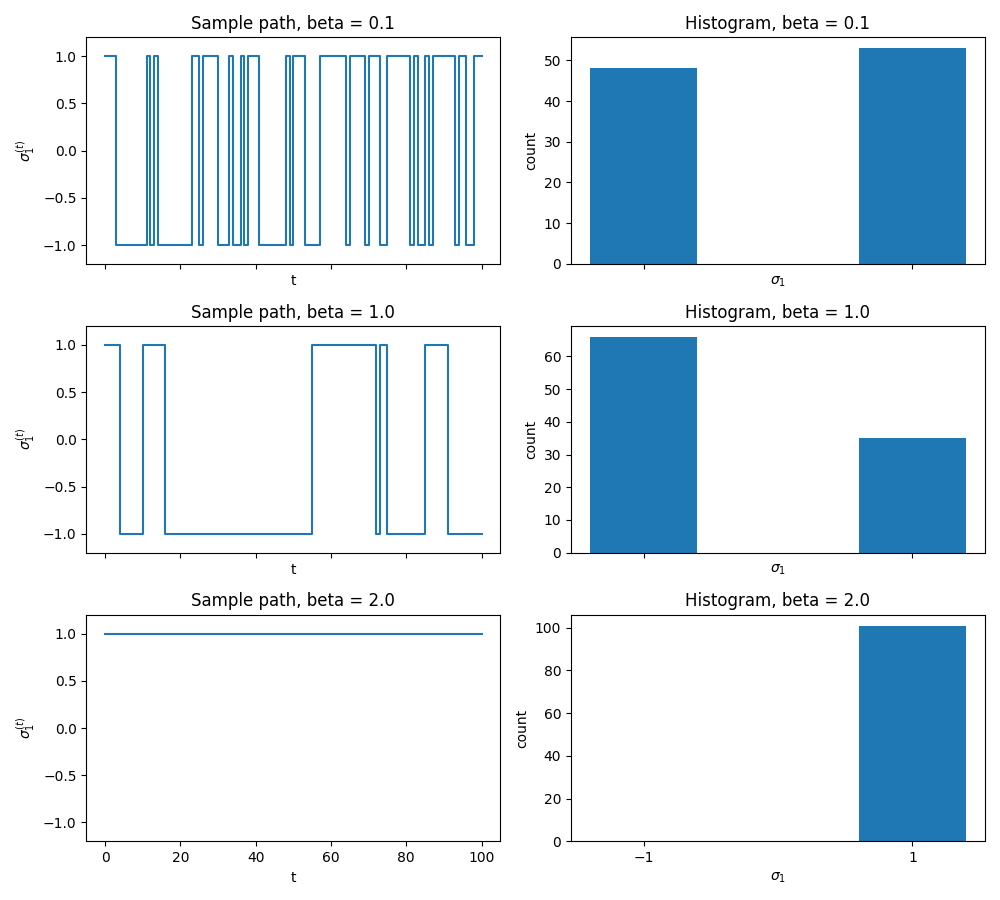
\includegraphics[width=0.9\textwidth]{hw4_2_4.png}
\end{center}

These empirical results are consistent with the theoretical spectral gap
from part (c): as $\beta$ increases (so $\rho=\tanh\beta\to 1$), the chain
mixes more slowly, resulting in longer runs and, for large $\beta$, very
slow movement away from the initial high-probability state.
\end{solution}
\end{enumerate}

%%%%%%%%%%%%%%%%%%%%%%%%%%%%%%%%%%%%%%%%%%%%%%%%
\section*{Problem 3: Gibbs sampler on a continuous state space}

Let $x_0, x_1, \ldots, x_n \in \mathbb{R}^d$. Suppose
\[
x_0 \sim p(x_0),
\]
where $p$ is an arbitrary probability density on $\mathbb{R}^d$. For $i = 0,1,\ldots,n-1$, suppose the forward diffusion process is given by
\[
x_{i+1} = a_i x_i + \xi_i, \qquad \xi_i \sim N(0, \sigma_i^2 I_d),
\]
independently across $i$. We observe
\[
y = x_0 + \varepsilon, \qquad \varepsilon \sim N(0, \tau^2 I_d),
\]
independently of everything else.

\begin{enumerate}
\item Show that the joint density of $(x_0, \ldots, x_n, y)$ is, up to a constant,
\[
p(x_0)
\exp\!\left(
-\frac{\|y - x_0\|^2}{2\tau^2}
\right)
\prod_{i=0}^{n-1}
\exp\!\left(
-\frac{\|x_{i+1} - a_i x_i\|^2}{2\sigma_i^2}
\right).
\]
\begin{solution}
We are given the hierarchical model
\[
x_0 \sim p(x_0), \qquad
x_{i+1} \mid x_i \sim N(a_i x_i,\sigma_i^2 I_d), \quad i=0,\dots,n-1,
\]
independently across $i$, and
\[
y \mid x_0 \sim N(x_0,\tau^2 I_d),
\]
independently of everything else.

By the chain rule for densities, the joint density of $(x_0,\ldots,x_n,y)$ can be written as
\[
p(x_0,\ldots,x_n,y)
= p(x_0)\,\prod_{i=0}^{n-1} p(x_{i+1} \mid x_i)\,p(y \mid x_0).
\]
Each conditional distribution is Gaussian with density
\[
p(x_{i+1} \mid x_i)
= \frac{1}{(2\pi\sigma_i^2)^{d/2}}
\exp\!\left(
-\frac{\|x_{i+1} - a_i x_i\|^2}{2\sigma_i^2}
\right),
\]
and
\[
p(y \mid x_0)
= \frac{1}{(2\pi\tau^2)^{d/2}}
\exp\!\left(
-\frac{\|y - x_0\|^2}{2\tau^2}
\right).
\]
Therefore,
\[
p(x_0,\ldots,x_n,y)
= p(x_0)\,
\left[
\prod_{i=0}^{n-1}
\frac{1}{(2\pi\sigma_i^2)^{d/2}}
\right]
\frac{1}{(2\pi\tau^2)^{d/2}}
\exp\!\left(
-\frac{\|y - x_0\|^2}{2\tau^2}
- \sum_{i=0}^{n-1} \frac{\|x_{i+1} - a_i x_i\|^2}{2\sigma_i^2}
\right).
\]
All multiplicative constants in front of the exponential can be absorbed into a single proportionality
constant. Hence, up to a constant factor,
\[
p(x_0,\ldots,x_n,y)
\propto
p(x_0)
\exp\!\left(
-\frac{\|y - x_0\|^2}{2\tau^2}
\right)
\prod_{i=0}^{n-1}
\exp\!\left(
-\frac{\|x_{i+1} - a_i x_i\|^2}{2\sigma_i^2}
\right),
\]
which is the desired expression.
\end{solution}
\item Assuming we have observed $y$, we are interested in sampling from the posterior density
\[
\pi(x_0, \ldots, x_n \mid y)
\]
using a Gibbs sampler.
\begin{enumerate}
\item Fix $i \in \{1, \ldots, n-1\}$. Show that the full conditional density of $x_i$ given all the other variables and $y$,
\[
\pi(x_i \mid x_0, \ldots, x_{i-1}, x_{i+1}, \ldots, x_n, y),
\]
is Gaussian. (Hint: The conditional distribution of $x_i$ only depends on $x_{i-1}$ and $x_{i+1}$. Then try to complete the square.)
\begin{solution}
Fix $i \in \{1,\dots,n-1\}$. We consider the full conditional density of $x_i$
given all other variables and $y$:
\[
\pi(x_i \mid x_0,\dots,x_{i-1},x_{i+1},\dots,x_n,y).
\]
From the joint density in the previous part, we know that, up to a constant,
\[
p(x_0,\dots,x_n,y)
\propto
p(x_0)
\exp\!\left(
-\frac{\|y - x_0\|^2}{2\tau^2}
\right)
\prod_{k=0}^{n-1}
\exp\!\left(
-\frac{\|x_{k+1} - a_k x_k\|^2}{2\sigma_k^2}
\right).
\]
In this product, the only factors that depend on $x_i$ are those with $k=i-1$
and $k=i$, namely
\[
\exp\!\left(
-\frac{\|x_i - a_{i-1} x_{i-1}\|^2}{2\sigma_{i-1}^2}
\right)
\quad\text{and}\quad
\exp\!\left(
-\frac{\|x_{i+1} - a_i x_i\|^2}{2\sigma_i^2}
\right).
\]
All other terms in the joint density are constant with respect to $x_i$ and can
be absorbed into the proportionality constant. Therefore the full conditional
density of $x_i$ is, up to a normalizing constant,
\[
\pi(x_i \mid \text{rest})
\propto
\exp\!\left(
-\frac{\|x_i - a_{i-1} x_{i-1}\|^2}{2\sigma_{i-1}^2}
-\frac{\|x_{i+1} - a_i x_i\|^2}{2\sigma_i^2}
\right).
\]

We now show this is a multivariate normal density in $x_i$ by completing the
square. Expanding the two quadratic terms and discarding all terms independent
of $x_i$, we obtain that the exponent equals
\[
-\frac{1}{2}
\left[
x_i^\top\left(\frac{1}{\sigma_{i-1}^2} I_d + \frac{a_i^2}{\sigma_i^2} I_d\right)x_i
- 2 x_i^\top\left(
\frac{a_{i-1}}{\sigma_{i-1}^2} x_{i-1}
+ \frac{a_i}{\sigma_i^2} x_{i+1}
\right)
\right]
+ \text{const}.
\]
Define
\[
\Lambda_i
= \left(
\frac{1}{\sigma_{i-1}^2}
+ \frac{a_i^2}{\sigma_i^2}
\right) I_d,
\qquad
b_i
= \frac{a_{i-1}}{\sigma_{i-1}^2} x_{i-1}
+ \frac{a_i}{\sigma_i^2} x_{i+1}.
\]
Completing the square,
\[
-\frac{1}{2}\left(x_i^\top \Lambda_i x_i - 2 x_i^\top b_i\right) + \text{const}
= -\frac{1}{2}(x_i - m_i)^\top \Lambda_i (x_i - m_i) + \text{const}',
\]
where
\[
m_i = \Lambda_i^{-1} b_i
= \frac{
\dfrac{a_{i-1}}{\sigma_{i-1}^2} x_{i-1}
+ \dfrac{a_i}{\sigma_i^2} x_{i+1}
}{
\dfrac{1}{\sigma_{i-1}^2} + \dfrac{a_i^2}{\sigma_i^2}
},
\qquad
\Sigma_i = \Lambda_i^{-1}
= \left(
\frac{1}{\sigma_{i-1}^2}
+ \frac{a_i^2}{\sigma_i^2}
\right)^{-1} I_d.
\]
Thus, the full conditional distribution of $x_i$ given all other variables and
$y$ is multivariate Gaussian:
\[
x_i \mid x_{i-1},x_{i+1},\text{rest}
\sim \mathcal{N}\bigl(m_i,\Sigma_i\bigr),
\]
with mean $m_i$ and covariance $\Sigma_i$ as above. In particular, the
conditional depends on the other variables only through $x_{i-1}$ and $x_{i+1}$,
as claimed.
\end{solution}
\item Show similarly that the last coordinate also has a Gaussian full conditional:
\[
x_n \mid x_0, \ldots, x_{n-1}, y \sim N(a_{n-1} x_{n-1}, \sigma_{n-1}^2 I_d).
\]
\begin{solution}
We consider the full conditional distribution of the last state $x_n$ given all
other variables and $y$:
\[
\pi(x_n \mid x_0,\dots,x_{n-1},y).
\]
From the joint density (up to a constant),
\[
p(x_0,\dots,x_n,y)
\propto
p(x_0)
\exp\!\left(
-\frac{\|y - x_0\|^2}{2\tau^2}
\right)
\prod_{i=0}^{n-1}
\exp\!\left(
-\frac{\|x_{i+1} - a_i x_i\|^2}{2\sigma_i^2}
\right),
\]
we see that $x_n$ appears only in the last transition factor with index $i=n-1$:
\[
\exp\!\left(
-\frac{\|x_n - a_{n-1} x_{n-1}\|^2}{2\sigma_{n-1}^2}
\right).
\]
All other factors in the joint density do not depend on $x_n$ and are therefore
constants with respect to $x_n$. Hence the full conditional is, up to a
normalizing constant,
\[
\pi(x_n \mid x_0,\dots,x_{n-1},y)
\propto
\exp\!\left(
-\frac{\|x_n - a_{n-1} x_{n-1}\|^2}{2\sigma_{n-1}^2}
\right).
\]
This is exactly the kernel of a multivariate normal distribution with mean
$a_{n-1} x_{n-1}$ and covariance $\sigma_{n-1}^2 I_d$. Therefore,
\[
x_n \mid x_0,\dots,x_{n-1},y
\sim N\bigl(a_{n-1} x_{n-1},\,\sigma_{n-1}^2 I_d\bigr),
\]
as claimed.
\end{solution}
\end{enumerate}
\end{enumerate}

%%%%%%%%%%%%%%%%%%%%%%%%%%%%%%%%%%%%%%%%%%%%%%%%
\section*{Problem 4: Independent Metropolis--Hastings}

Let $\Omega = \{1, 2, \ldots, n\}$ be a finite state space. Suppose the target distribution is
\[
\pi = (\pi_1, \ldots, \pi_n),
\]
and suppose we are able to sample from another distribution
\[
p = (p_1, \ldots, p_n),
\]
where $\pi_i > 0$ and $p_i > 0$ for every $i$.

Consider the following independent Metropolis--Hastings sampler. If the current state is $X_t = i$, then:
\begin{enumerate}
\item propose a new state $J$ from the distribution $p$, independently of the current state;
\item accept the proposal with probability
\[
\alpha(i,J) = \min\left(1,\frac{\pi_J p_i}{\pi_i p_J}\right);
\]
otherwise, stay at $i$.
\end{enumerate}

Define
\[
w_i = \frac{\pi_i}{p_i}, \quad i = 1,\ldots,n,
\]
and assume, without loss of generality, that
\[
w_1 \ge w_2 \ge \cdots \ge w_n.
\]

\begin{enumerate}
\item Show that for $i \neq j$,
\[
P(i,j) =
\begin{cases}
p_j, & \text{if } j < i,\\[4pt]
\displaystyle \frac{p_j}{w_j} w_i, & \text{if } j > i.
\end{cases}
\]
Also write down a formula for $P(i,i)$.
\begin{solution}
Recall the independent Metropolis--Hastings update: if $X_t = i$, we propose
$J \sim p$ independently of $i$ and accept the proposal with probability
\[
\alpha(i,J)
= \min\!\left(1,\frac{\pi_J p_i}{\pi_i p_J}\right)
= \min\!\left(1,\frac{w_J}{w_i}\right),
\]
where $w_k = \pi_k/p_k$ for $k=1,\dots,n$. Thus the one-step transition
probabilities are
\[
P(i,j)
= \mathbb{P}(X_{t+1}=j \mid X_t=i)
=
\begin{cases}
p_j\,\alpha(i,j), & j \neq i,\\[4pt]
1 - \displaystyle\sum_{k\neq i} p_k\,\alpha(i,k), & j = i.
\end{cases}
\]

We now use the ordering assumption $w_1 \ge w_2 \ge \cdots \ge w_n$ to simplify
$\alpha(i,j)$ according to whether $j<i$ or $j>i$.

\medskip
\noindent\textbf{Case $j < i$.}
Since the weights are nonincreasing, $j<i$ implies $w_j \ge w_i$. Hence
\[
\frac{w_j}{w_i} \ge 1
\quad\Longrightarrow\quad
\alpha(i,j) = \min\!\left(1,\frac{w_j}{w_i}\right)
= 1.
\]
Therefore, for $j<i$,
\[
P(i,j) = p_j\,\alpha(i,j) = p_j.
\]

\medskip
\noindent\textbf{Case $j > i$.}
Now $j>i$ implies $w_j \le w_i$, so
\[
\frac{w_j}{w_i} \le 1
\quad\Longrightarrow\quad
\alpha(i,j) = \min\!\left(1,\frac{w_j}{w_i}\right)
= \frac{w_j}{w_i}.
\]
Thus for $j>i$,
\[
P(i,j) = p_j\,\alpha(i,j)
= p_j\,\frac{w_j}{w_i}.
\]

Combining the two cases, for $i\neq j$ we have
\[
P(i,j) =
\begin{cases}
p_j, & j < i,\\[4pt]
\displaystyle p_j\,\frac{w_j}{w_i}, & j > i,
\end{cases}
\]
as required.

\medskip
\noindent\textbf{Formula for $P(i,i)$.}
Finally, the probability of staying at $i$ is one minus the probability of
moving to any other state:
\[
P(i,i)
= 1 - \sum_{j\neq i} P(i,j)
= 1 - \sum_{j<i} p_j - \sum_{j>i} p_j\,\frac{w_j}{w_i}.
\]
This gives an explicit expression for $P(i,i)$ in terms of $\{p_j,w_j\}$.
\end{solution}
\item Show that
\[
P = U + R,
\]
where $R$ is a rank-one matrix and $U$ is upper triangular. In particular, show that the diagonal
entries of $U$ are
\[
U_{ii} = \sum_{j>i} p_j\left(1 - \frac{w_j}{w_i}\right),
\qquad i = 1,\ldots,n.
\]
(Hint: Try subtracting the vector $(p_1, p_2, \ldots, p_n)$ from every row of $P$.)
\begin{solution}
From part (1), for $i \neq j$ we have
\[
P(i,j) =
\begin{cases}
p_j, & j < i,\\[4pt]
p_j \dfrac{w_j}{w_i}, & j > i,
\end{cases}
\]
and
\[
P(i,i) = 1 - \sum_{j<i} p_j - \sum_{j>i} p_j \frac{w_j}{w_i}.
\]

\medskip
\noindent\textbf{Decomposition $P = U + R$.}
Define the matrix $R$ to be the rank-one matrix
\[
R_{ij} = p_j, \qquad i,j = 1,\dots,n.
\]
That is, $R$ has the same row vector $(p_1,\dots,p_n)$ in every row. Then define
\[
U = P - R.
\]
By construction, $R$ clearly has rank one (it is the outer product of the all-ones
vector with the row vector $(p_1,\dots,p_n)$), and we have $P = U + R$.

We now compute the entries of $U$. For $i \neq j$,
\[
U(i,j) = P(i,j) - p_j =
\begin{cases}
p_j - p_j = 0, & j < i,\\[6pt]
p_j \dfrac{w_j}{w_i} - p_j = p_j\!\left(\dfrac{w_j}{w_i} - 1\right)
= -\,p_j\!\left(1 - \dfrac{w_j}{w_i}\right), & j > i.
\end{cases}
\]
Thus $U(i,j) = 0$ whenever $j < i$, so $U$ is upper triangular. For $j>i$, the
entries $U(i,j)$ may be nonzero, but they appear only above the diagonal.

For the diagonal entries,
\[
U(i,i) = P(i,i) - p_i
= \left( 1 - \sum_{j<i} p_j - \sum_{j>i} p_j \frac{w_j}{w_i} \right) - p_i.
\]
Rewriting $1 - \sum_{j<i} p_j - p_i = \sum_{j>i} p_j$, we obtain
\[
U(i,i)
= \sum_{j>i} p_j - \sum_{j>i} p_j \frac{w_j}{w_i}
= \sum_{j>i} p_j\left(1 - \frac{w_j}{w_i}\right).
\]

\medskip
We have therefore decomposed $P$ as
\[
P = U + R,
\]
where $R$ is rank one, $U$ is upper triangular (since $U(i,j)=0$ for $j<i$), and the
diagonal entries of $U$ are
\[
U_{ii} = \sum_{j>i} p_j\left(1 - \frac{w_j}{w_i}\right), \qquad i=1,\dots,n,
\]
as required.
\end{solution}
\item (Rank-one perturbation) Suppose $A$ is an $n \times n$ real matrix with real eigenvalues
\[
\lambda_1, \ldots, \lambda_n
\]
and corresponding real eigenvectors
\[
u_1, \ldots, u_n.
\]
Let $u \in \mathbb{R}^n$ be any vector such that
\[
\lambda_i - \lambda_n - u^\top u_n \neq 0
\quad \text{for all } i = 1,\ldots, n-1.
\]
Define
\[
B = A + u_n u^\top.
\]
Then $B$ has eigenvalues
\[
\lambda_1, \lambda_2, \ldots, \lambda_{n-1},\ \lambda_n + u^\top u_n,
\]
with corresponding eigenvectors
\[
\tilde{u}_j =
\begin{cases}
u_n, & \text{if } j = n,\\[4pt]
u_j + c_j u_n, & \text{if } j \neq n,
\end{cases}
\]
where
\[
c_j = \frac{u^\top u_j}{\lambda_j - \lambda_n - u^\top u_n}.
\]
\begin{solution}
Let $A$ be an $n\times n$ real matrix with real eigenvalues
$\lambda_1,\dots,\lambda_n$ and corresponding eigenvectors
$u_1,\dots,u_n$. Let $u\in\mathbb{R}^n$ be such that
\[
\lambda_i - \lambda_n - u^\top u_n \neq 0 \quad \text{for all } i=1,\dots,n-1.
\]
Define the rank-one perturbation
\[
B = A + u_n u^\top.
\]
We show that $B$ has eigenvalues
$\lambda_1,\dots,\lambda_{n-1},\lambda_n + u^\top u_n$ with
corresponding eigenvectors
\[
\tilde u_j =
\begin{cases}
u_n, & j = n,\\[0.3em]
u_j + c_j u_n, & j \neq n,
\end{cases}
\qquad
c_j = \dfrac{u^\top u_j}{\lambda_j - \lambda_n - u^\top u_n}.
\]

\medskip\noindent
\emph{Case $j = n$.}
Take $\tilde u_n = u_n$. Then
\[
B \tilde u_n
= (A + u_n u^\top) u_n
= A u_n + u_n (u^\top u_n)
= \lambda_n u_n + (u^\top u_n) u_n
= (\lambda_n + u^\top u_n) u_n.
\]
Thus $u_n$ is an eigenvector of $B$ with eigenvalue
$\lambda_n + u^\top u_n$.

\medskip\noindent
\emph{Case $j \neq n$.}
For $j \neq n$, define
\[
\tilde u_j = u_j + c_j u_n,
\]
with $c_j$ to be chosen so that $\tilde u_j$ is an eigenvector of $B$
with eigenvalue $\lambda_j$.

Compute $B \tilde u_j$:
\begin{align*}
B \tilde u_j
&= (A + u_n u^\top)(u_j + c_j u_n) \\
&= A u_j + c_j A u_n + u_n u^\top u_j + c_j u_n u^\top u_n \\
&= \lambda_j u_j + c_j \lambda_n u_n
+ u_n (u^\top u_j) + c_j u_n (u^\top u_n).
\end{align*}
Group terms in the basis $\{u_j,u_n\}$:
\[
B \tilde u_j
= \lambda_j u_j
+ u_n\bigl(c_j \lambda_n + u^\top u_j + c_j u^\top u_n\bigr).
\]

On the other hand, if $\tilde u_j$ is an eigenvector of $B$ with
eigenvalue $\lambda_j$, then
\[
B \tilde u_j = \lambda_j \tilde u_j
= \lambda_j (u_j + c_j u_n)
= \lambda_j u_j + c_j \lambda_j u_n.
\]
Comparing coefficients of $u_j$ and $u_n$ gives:
\[
c_j \lambda_n + u^\top u_j + c_j u^\top u_n = c_j \lambda_j.
\]
Rearranging,
\[
u^\top u_j
= c_j\bigl(\lambda_j - \lambda_n - u^\top u_n\bigr),
\]
and hence
\[
c_j = \frac{u^\top u_j}{\lambda_j - \lambda_n - u^\top u_n}.
\]
By assumption, the denominator is nonzero for all $j=1,\dots,n-1$, so
each $c_j$ is well-defined. Therefore, for every $j\neq n$, the vector
$\tilde u_j = u_j + c_j u_n$ is an eigenvector of $B$ with eigenvalue
$\lambda_j$.

\medskip
Combining the two cases, $B$ has eigenvalues
$\lambda_1,\dots,\lambda_{n-1},\lambda_n + u^\top u_n$ with
corresponding eigenvectors as claimed.
\end{solution}
\item Apply this fact to the decomposition
\[
P = U + R
\]
from the previous part, where $R$ is rank one, to derive the eigenvalues of $P$. (Hint: The eigenvalues of an upper triangular matrix are precisely its diagonal entries.)
\begin{solution}
From part (2), we have decomposed the transition matrix as
\[
P = U + R,
\]
where $R$ is rank one and $U$ is upper triangular with diagonal entries
\[
U_{ii} = \sum_{j>i} p_j\Bigl(1 - \frac{w_j}{w_i}\Bigr), \qquad i = 1,\dots,n.
\]
Since $U$ is upper triangular, its eigenvalues are precisely its diagonal
entries:
\[
\lambda_i(U) = U_{ii},\qquad i = 1,\dots,n.
\]

Next we identify $R$ in the form required by the rank-one perturbation lemma.
By definition,
\[
R_{ij} = p_j,\qquad i,j = 1,\dots,n,
\]
so every row of $R$ is equal to the row vector $(p_1,\dots,p_n)$.
Equivalently,
\[
R = {\bf 1}\, p^{\top},
\]
where ${\bf 1} = (1,\dots,1)^{\top}\in\mathbb{R}^n$ and
$p = (p_1,\dots,p_n)^{\top}$. Thus $R$ has rank one and can be written
in the form
\[
R = u_n u^{\top} \quad\text{with}\quad u_n = {\bf 1},\ u = p.
\]

We now apply the rank-one perturbation lemma from part (3) with
\[
A = U,\quad B = P = U + R,\quad u_n = {\bf 1},\quad u = p.
\]
The lemma states that $P$ has eigenvalues
\[
\lambda_1(U),\dots,\lambda_{n-1}(U),\ \lambda_n(U) + u^{\top}u_n,
\]
i.e.\ all but one of the eigenvalues of $U$ remain unchanged, and a single
eigenvalue is shifted by the amount
\[
u^{\top}u_n = p^{\top}{\bf 1} = \sum_{j=1}^n p_j = 1,
\]
since $p$ is a probability distribution. Hence the shifted eigenvalue equals
$\lambda_n(U) + 1$.

Because $P$ is a Markov transition matrix, it must have eigenvalue $1$;
therefore $\lambda_n(U) + 1 = 1$ and $\lambda_n(U) = 0$. The remaining
eigenvalues of $P$ are exactly the other diagonal entries of $U$:
\[
\lambda_i(P) = U_{ii},\qquad i = 1,\dots,n-1,
\]
up to a relabeling of indices. In particular, the full multiset of eigenvalues
of $P$ is
\[
\{1\} \cup \{U_{11},\dots,U_{n-1,n-1}\}.
\]
\end{solution}
\item Calculate the spectral gap of this independent Metropolis--Hastings chain.
\begin{solution}
From part (4), the eigenvalues of $P$ consist of
\[
1 \quad\text{and}\quad U_{11},\dots,U_{n-1,n-1},
\]
where all nontrivial eigenvalues (those different from $1$) are the diagonal
entries $U_{ii}$ for $i = 1,\dots,n-1$.

Recall from part (2) that
\[
U_{ii} = \sum_{j > i} p_j \Bigl(1 - \frac{w_j}{w_i}\Bigr),
\qquad i = 1,\dots,n,
\]
where $w_1 \ge \cdots \ge w_n$ by assumption. For $j>i$ we have
$w_j \le w_i$, so $1 - w_j/w_i \ge 0$ and hence each $U_{ii} \ge 0$.

For a reversible Markov chain with transition matrix $P$, the spectral gap
is defined as
\[
\gamma
= 1 - \max\{|\lambda| : \lambda \text{ eigenvalue of } P,\ \lambda \neq 1\}.
\]
Using the description above and the fact that all nontrivial eigenvalues are
nonnegative, we obtain
\[
\gamma
= 1 - \max_{1 \le i \le n-1} U_{ii}
= 1 - \max_{1 \le i \le n-1}
\sum_{j > i} p_j \Bigl(1 - \frac{w_j}{w_i}\Bigr).
\]
This expression gives the spectral gap of the independent
Metropolis--Hastings chain in terms of the proposal probabilities $(p_j)$ and
weights $(w_j)$.
\end{solution}
\end{enumerate}

\end{document}
